\subsubsection{Частотно-временной анализ} 

Аналогично формализации SSA (\myref{link::ssa}), также рассматриваем  второе определение стационарности (\myref{def::signal_stationarity}), предполагающее отношение к сигналу как набору величин, характеризующих некоторый объект на промежутке времени. Ключевой особенностью рассматриваемого в текущем блоке подхода - анализа Фурье - является <<сканирование>> исходных сигналов в частотном пространстве, а не временн\'{о}м, в котором данные изначально представлены. \textbf{Q}: Каким образом осуществляется переход подобного рода? \textbf{A}: Описано далее. Однако помним, что теперь сигнал, будучи характеристикой некоторого объекта может быть непрерывен, что уводит нас от дискретного анализа, как было в случае подхода ARIMA и GARCH (ARFIMA и FIGARCH уже немного залезли в непрерывную область с точки зрения лагов), к непрерывному. Обратный переход делается при построении и рассмотрении алгоритма Быстрого Преобразования Фурье (Fast Fourier Transform - FFT) (\myref{link::fft}), где для корректной работы алгоритма как такового требуется переход к дискретности. 

Из непрерывности сигнала следует факт, что теперь сигнал - это некоторая функцию $f: \R \to \R$, от переменной $t$ - время. Более того, пока что не делаем никаких предположений относительно поведения $f(t)$, то есть она, конечно, непрерывна, иначе разрыв характеризовался бы потерей соединения с записывающим устройством, но о наклонах, изгибах и так далее предположения пока что не выдвигаются.

Теперь переходим непосредственно к блоку анализа Фурье, где объясняется принцип и необходимость перехода к частотному (только частотному, а не частотно-временному) пространству.

\subsubsubsection{Анализ Фурье} \label{link::fourier_analysis}
\\\\
\indent По изначальному подходу, сигнал $f(t)$ - это некоторая функция, то есть ее можно пытаться чем-то приближать. Конечно, далеко не всякую функцию можно аппроксимировать, однако пока что оставляем математическую строгость за кадром и просто пробуем. Но в таком случае из чего-то сложного как исходный сигнал, получаем что-то более простое, но поддающееся анализу, значит, мы раскладываем имеющуюся $f(t)$ на простые составляющие. Замечаем, что в первом приближении для этого должны быть выбраны простые функции, которые легко поддаются анализу. В таком случае, задаемся вопросом~\textbf{Q}: Можно ли как-то представить функцию вида $f(t)$ (исследуемый непрерывный сигнал) в виде конечного или бесконечного наложения синусоид (под синусоидой понимается как косинус, так и синус). \textbf{A}:~1)~Замечаем, что существует неточность: почему именно синусоиды? \textbf{Q}:~Почему нельзя взять иной набор функций, на которые раскладывается сигнал? \textbf{A}: Любой набор взять нельзя, однако при определенных условиях подобный подход приводит к рассматриваемому далее Wavelet анализу (\myref{link::wavelet_analysis}). На данный момент останавливаем рассуждения на  упоминании синусоид. Изначально было отмечено \cite{mipt2021string}, что струна - это тонкая и гибкая нить, способная совершать колебания при условии фиксированных концов как раз на основе синусоидальных форм. Причем по всей длине струны всегда умещается конечное количество волн. Это обеспечивается условием закрепленности струны на обоих концах. 

Самая простая форма колебания струны называется "гармоникой". Отсюда и происходит второе название анализа Фурье - гармонический анализ. Таким образом, формализуя исходную задачу, получаем выражение (\ref{equation::fourier_approximation}). Отмечаем, что факт того, как данное выражение изначально получено находится за областью, исследуемой в настоящей работе. Следовательно, предполагаем, что подобная форма разложения в ряд Фурье была <<угадана>>. 
\begin{equation} \label{equation::fourier_approximation}
	f(t) = \frac{a_0}{2} + \sum_{k = 1}^{\infty} a_k\cos(k \omega t) + b_k\sin(k \omega t)
\end{equation}
\indent Однако, несмотря на вольность предположений, далее совершенно строго находим для данного разложения все необходимые коэффициенты. Более того, отмечаем, что пока не было введено никаких предпосылок относительно $f(t)$, но далее они потребуются.

Пусть исходный сигнал $f(t)$ является периодическим с периодом $T$, тогда, основываясь на знаниях из Линейной Алгебры об ортогональных векторах, по аналогии вводим операцию <<измеряющую степень>> ортогональности функций~\cite{penn2016orthogonal}. В итоге получаем:
\begin{equation}
	p = \int_0^T g(t) f(t) \; \text{d}t
\end{equation}
\indent Далее вычисляем данную меру для выбранных в качестве базисных функций $\cos(\cdot)$ и $\sin(\cdot)$. Если $p \ne 0$, то вся проводимая операция не может быть названа разложением по базисным функциям. В силу того, что под <<синусоидой>> подразумевается как $\sin(\cdot)$, так и $\cos(\cdot)$, вычисляем меру $p$ для каждого из четырех возможных вариантов их комбинаций.
\begin{enumerate}
	\item $\sin(k\omega t), \sin(l \omega t): k, l \in \N, \omega \in \R^+$.
	\begin{equation}
		p = \int_{0}^T \sin(k\omega t)\sin(l \omega t) \; dt =
		\left\{
		\begin{array}{rl}
			0 & \text{, } k \ne l\\
			T / 2 & \text{, } k = l
		\end{array}
		\right.
	\end{equation}
	
	\item $\cos(k\omega t), \cos(l \omega t): k, l \in \N, \omega \in \R^+$.
	\begin{equation}
		p = \int_{0}^T \cos(k\omega t)\cos(l \omega t) \; dt =
		\left\{
		\begin{array}{rl}
			0 & \text{, } k \ne l\\
			T / 2 & \text{, } k = l
		\end{array}
		\right.
	\end{equation}
	
	\item $\cos(k\omega t), \sin(l \omega t): k, l \in \N, \omega \in \R^+$.
	\begin{equation}
		p = \int_{0}^T \cos(k\omega t)\sin(l \omega t) \; dt = 0
	\end{equation}
\end{enumerate}
Тогда, опираясь на  выражение (\ref{equation::fourier_approximation}) и умножение его обеих частей на $\sin(k\omega t)$ и $\cos(l \omega t)$, получаем формулы для коэффициентов. Рассматриваем только для $\sin(\cdot)$, так как аналогичным образом получается для $\cos(\cdot)$.
\begin{equation}
	\int_{0}^T f(t) \sin(p \omega t) dt = \int_0^T \sin(p \omega t) \left(\sum_{k = 1}^{\infty} a_k\cos(k \omega t) + b_k\sin(k \omega t) \right) dt
\end{equation}
Однако изменять порядок интегрирования и суммирования, при условии бесконечной суммы, можно только в случае равномерной сходимости ряда. Для настоящего ряда проблем в сходимости не наблюдается \cite{teljacovski2001convergence}, \cite{mipt2004fourier}. Преобразуем выражение, приняв во внимание факт ортогональности функций, описанный выше:
\begin{equation}
	\begin{split}
		\int_{0}^T f(t) \sin(p \omega t) \; dt & = \sum_{k = 1}^{\infty} b_k \int_0^T \sin(k \omega t)\sin(p \omega t) \; dt = T / 2  \cdot b_p \\
		b_k & = \frac{2}{T}  \int_{0}^T f(t) \sin(k \omega t) \; dt 
	\end{split}
\end{equation}
Аналогичным образом получаем выражение для коэффициентов $a_k$:
\begin{equation}
	a_k = \frac{2}{T}  \int_{0}^T f(t) \cos(k \omega t) \; dt 
\end{equation}
В более удобной форме вся задача приближения выглядит:
\begin{equation} \label{eq::fourier_task}
	\begin{split}
		f(t) & = \frac{a_0}{2} + \sum_{k = 1}^{\infty} a_k\cos(k \omega t) + b_k\sin(k \omega t)\\
		& = \frac{a_0}{2} + \sum_{k = 1}^{\infty} A_k \cos(k \omega t - \phi_k)\\
		A_k & = \sqrt{a_k^2 + b_k^2}\\
		\phi_k & = \arctan(b_k / a_k)\\
	\end{split}
\end{equation}
Где $A_k$ - амплитуда сигнала, а набор амплитуд $\left\{A_k\right\}_{k = 1}^\infty$ - спектр сигнала, $\phi_k$ - фаза сигнала. Переход к подобной записи как после 2-ого знака равенства сделан для того, чтобы было интуитивно удобнее характеризовать величину посредством не синуса и косинуса, а амплитуды и фазы в конкретный момент времени. Однако (\ref{eq::fourier_task}) можно еще больше упростить, перейдя в комплексную плоскость и воспользовавшись тождеством Эйлера:
\begin{equation}
	\exp(i k \omega t) = \cos(k \omega t) + i \sin(k \omega t)
\end{equation}
Отсюда получаем выражения для $\cos(k \omega t)$ и $\sin(k \omega t)$, после чего переписываем не все приближение, а только конкретный коэффициент $k$ (это сделано для удобства восприятия):
\begin{equation}
	\begin{split}
		a_k \cdot \frac{\exp(i k \omega t) + \exp(-i k \omega t)}{2} & + b_k \cdot \frac{\exp(i k \omega t) - \exp(-i k \omega t)}{2i}\\
		\underbrace{\left( \frac{a_k}{2} - \frac{b_k}{2} i \right) \exp(i k \omega t)}_{\text{<<Положительная>> часть}} & + \underbrace{\left( \frac{a_k}{2} + \frac{b_k}{2} i \right) \exp(-i k \omega t)}_{\text{<<Отрицательная>> часть}}
	\end{split}
\end{equation}
Отсюда получаем:
\begin{equation}
	c_k = \left\{
	\begin{array}{rl}
		a_k / 2 - i \cdot b_k/ 2  & \text{ ; } k \ge 0\\ 
		a_k / 2 + i \cdot b_k/ 2  & \text{ ; } k < 0\\ 
	\end{array}
	\right.
\end{equation}
В конечно виде (\ref{eq::fourier_task}) записывается уже как:
\begin{equation}
	f(t) = \sum_{k = -\infty}^{\infty} c_k \exp(i k \omega t)
\end{equation}
Однако тут интерес представляют сами коэффициенты $c_k$, так как именно они и являются коэффициентами Фурье при проецировании на базисные функции. 
\begin{equation}
	\begin{split}
		c_k & = \frac{a_k - i b_k}{2} = \frac{1}{\cancel{2}} \frac{\cancel{2}}{T} \int_0^T f(t) \cos(k \omega t) - f(t) \sin(k \omega t) \; dt\\
		& = \frac{1}{2 T} \int_{-T}^T f(t) \exp(-i k \omega t) \; dt
	\end{split}
\end{equation}
Вспоминаем, что ранее вводилась предпосылка, относительно периодичности сигнала $f(t)$. \textbf{Q}: Как быть в противном случае? \textbf{A}: Необходимо сам период устремить к $\infty$. Но прежде подставляем вместо некоторой частоты $\omega$ конкретное значение: $\omega = k \Delta \omega$, где $\Delta \omega = \pi / T$. Следовательно, $c_k = \langle f, \psi_k\rangle / (2 \pi)$, где $\psi_k \equiv \exp(i k t)$. Значит:
\begin{equation}
	\begin{split}
		f(t) & = \lim_{\Delta \omega \to 0} \sum_{k = -\infty}^{\infty} \frac{\Delta \omega}{2 \pi} \left[\int_{-\pi / \Delta \omega}^{\pi / \Delta \omega} f(\xi) \exp(-i k \Delta \omega \xi) \; d \xi\right] \exp(i k \Delta \omega)\\
	\end{split}	
\end{equation}
Но подобное выражение, путем вычисления предела, превращается в:
\begin{equation}
	\begin{split}
		f(t) & = \int_{-\infty}^{\infty} \frac{1}{2\pi} \underbrace{\left\{\int_{-\infty}^{\infty} f(\xi) \exp(-i \omega \xi) \; d \xi \right\}}_{\hat{f}(\omega)} \exp(i \omega t) \; d \omega\\
		f(t) & = \frac{1}{2 \pi} \int_{-\infty}^{\infty} \hat{f}(\omega) \exp(i \omega t) \; d\omega
	\end{split}
\end{equation}
Вывод: получаются формулы для прямого и обратного преобразования Фурье.
\begin{equation}
	\begin{split}
		\hat{f}(\omega) & = \mathcal{F}(f(t)) = \int_{-\infty}^{\infty} f(t) \exp(-i \omega t) \; dt\\
		f(t) & = \mathcal{F}^{-1}(\hat{f}(\omega)) = \frac{1}{2 \pi} \int_{-\infty}^{\infty} \hat{f}(\omega) \exp(i \omega t) \; d\omega
	\end{split}
\end{equation}
Таким образом, получаем возможность анализа функции в частотном пространстве. Однако стоит упомянуть, что преобразование Фурье имеет смысл применять только в случае стационарного спектра сигнала. То есть, как говорится в (\myref{def::signal_stationarity}), набор частот не должен меняться во времени. 

\begin{theorem}[теорема Персеваля \cite{brunton2022data}] \label{thm::parceval}
	<<Энергия>> исходного сигнала $f(t)$ (если он не является периодическим) или его <<сила>> (в случае периодичности) в пространстве времени $(t)$ равна данной величине, но в пространстве частот~$(\omega)$. 
	\begin{equation}
		\int_{\R} \lvert f(t) \rvert ^2 \; dt = \int_{\R} \lvert \hat{f}(\omega) \rvert ^2 \; d \omega
	\end{equation}
	В случае ненормированности базисной функции:
	\begin{equation}
		\lVert \hat{f} \rVert^2 = 2 \pi \lVert f \rVert^2 \Rightarrow \lVert \hat{f} \rVert^2 \propto \lVert f \rVert^2
	\end{equation}
	Где $\lVert f \rVert^2 = \int_{-\infty}^{\infty} \lvert f(t) \rvert^2 \; dt$.
\end{theorem}
Иными словами, данная теорема утверждает: если есть коэффициенты Фурье, которые достаточно малы (то есть по модулю близки к $0$), то <<удалив>> их (приравняв к $0$) получаем сигнал близкий к исходному $f(t)$.
\subsubsubsection{Быстрое преобразование Фурье} \label{link::fft}
\\\\
\subsubsubsection{Пример: FFT удаление шума}
\\\\
\indent Основываясь на теореме (\myref{thm::parceval}), приводим в качестве примера решение задачи об удалении шума. К сожалению, в силу постоянства спектра сигнала, данные, исследуемые в блоке (\myref{link::mssa}) в качестве примера для сравнения использовать не получится, так как ключевой их особенностью является наличие трендовой составляющей. Следовательно с течение времени частота сигнала изменяется, однако предположив периодичность каждый $[-5, 5]$, получаем возможность приблизить на данном отрезке функцию. Следовательно, можем перейти в пространство частот для данного участка. То есть ничто не мешает технически вычислить коэффициенты Фурье и, основываясь на них, <<очистить>> исходную функцию от шума.
\begin{figure}[H]
	\centering
	\begin{tikzpicture}
		\begin{axis}[
			grid = both,
			legend pos = north west,
			minor tick num = 1,
			major grid style = {lightgray},
			minor grid style = {lightgray!25},
			%title= {},
			width = \textwidth,
			height = 0.45 \textwidth,
			xmin=-5, xmax=5,
			ymin=-4, ymax=7.5,
			line width=0.3mm
			]
			
			\addplot[color = orange, line width = 0.035cm] table [
			x=x, 
			y=y_clean, 
			col sep=comma,
			mark={},
			] {./source/source_csv/Illustration data/fft/denoised_data_incorrect.csv};
			
			\addplot[opacity = 0.25, color = blue] table [
			x=x, 
			y=y_initial, 
			col sep=comma,
			mark={},
			] {./source/source_csv/Illustration data/fft/denoised_data_incorrect.csv};
			
			\addplot[domain = -5:5,
			samples = 300,
			color = teal,
			smooth,
			line width = 0.025cm,] {sin(deg(5 * x)) + 1 / 4 * (x^2)};
			
			\legend{$f(x)$ очищенный, $f(x)$ c шумом, $f(x)$ без шума};
		\end{axis}
	\end{tikzpicture}
	\caption{Очистка ряда от шума посредством преобразования Фурье}
\end{figure}
Из графика видим, что восстановление прошло намного лучше, чем было изначально представлено в (\myref{link::mssa}), что обусловлено цикличностью данного отрезка, то есть спрогнозировать что-либо новое за пределами восстановленной области (дальше, чем $[-5, 5]$) не получится, так как все, что дальше - это повтор того, что находится на данном отрезке. Настоящий ряд, в котором отсутствует шум был восстановлен через  использование первых $8$-и частот, показавших наибольшие амплитуды.

Более того, график зависимости качества восстановления от количества использованных частот имеет вид:
\begin{figure}[H]
	\centering
	\begin{tikzpicture}
		\begin{axis}[
			grid = both,
			legend pos = north west,
			minor tick num = 1,
			major grid style = {lightgray},
			minor grid style = {lightgray!25},
			%title= {},
			width = \textwidth,
			height = 0.45 \textwidth,
			xmin=1, xmax=80,
			ymin=-4, ymax=7.5,
			line width=0.3mm
			]
			
			\addplot[line width = 0.035cm] table [
			x=k, 
			y=rmse, 
			col sep=comma,
			mark={},
			] {./source/source_csv/Illustration data/fft/statisticalDataRMSE.csv};
			\addplot +[mark=none] coordinates {(8, -4) (8, 8)};
			
			\node at (250,600) {$k = 8$, RMSE$(8) = 0.079$};
			
			\draw[->] (110,600) -- (75, 450);
			\legend{$k$ - количество использованных частот};
		\end{axis}
	\end{tikzpicture}
	\caption{RMSE$(k)$ - ошибка Root Mean Squared Error для восстановленного ряда относительно истинного ряда без шума. RMSE = $\sqrt{\text{MSE}} = \sqrt{1 / n \sum(\hat{y}_j - y_j)^2}$}
\end{figure}
Однако, несмотря на такой хороший результат, нельзя забывать, что 1) у преобразования Фурье существует гиперпараметр, отвечающий за количество используемых для восстановления частот 2) исходная функция (без шума) в реальности почти всегда не является наблюдаемой, то есть не от чего отталкиваться, чтобы измерить ошибку RMSE. А значит, на данный моменты в настоящей работе MSSA остается лидером в вопросе непараметризованной очистки данных от шума.

В качестве более удачного примера рассматриваем функцию вида:
\begin{equation} \label{link::new_function}
	f(t) = 1.25 \sin(3x) + 2\cos(4x) + 2.5 \cdot \varepsilon: \; \varepsilon \sim N(0, I_n)
\end{equation}
Изначально график функции с уже примененным алгоритмом очистки путем преобразования Фурье имеет вид:
\begin{figure}[H]
	\centering
	\begin{tikzpicture}
		\begin{axis}[
			grid = both,
			legend pos = north west,
			minor tick num = 1,
			major grid style = {lightgray},
			minor grid style = {lightgray!25},
			%title= {},
			width = \textwidth,
			height = 0.45 \textwidth,
			xmin=-5, xmax=5,
			ymin=-10, ymax=10,
			line width=0.3mm
			]
			
			\addplot[opacity= 0.3, color= purple] table [
			x=x, 
			y=y_initial, 
			col sep=comma,
			mark={},
			] {./source/source_csv/Illustration data/fft/denoised_data_correct.csv};
			
			\addplot[domain = -5:5,
			samples = 300,
			color = teal,
			smooth,
			line width = 0.025cm,] {1.25 * sin(deg(3 * x)) + 2 * cos(deg(4 * x))};
			
			\addplot table [
			x=x, 
			y=y_clean, 
			col sep=comma,
			mark={},
			] {./source/source_csv/Illustration data/fft/denoised_data_correct.csv};
						

			\legend{$f(t)$ с шумом, $f(t)$ без шума, $f(t)$ очищенная};
		\end{axis}
	\end{tikzpicture}
	\caption{Построение функции $(\ref{link::new_function})$}
\end{figure}
В свое время график амплитуд, имеет вид:
\begin{figure}[H]
	\centering
	\begin{tikzpicture}
		\begin{axis}[
			grid = both,
			legend pos = north west,
			minor tick num = 1,
			major grid style = {lightgray},
			minor grid style = {lightgray!25},
			%title= {},
			width = \textwidth,
			height = 0.35 \textwidth,
			xmin=0, xmax=0.05,
			ymin=0, ymax=0.9,
			line width=0.3mm,
			xlabel= Частота,
			ylabel= Амплитуда
			]
			
			\addplot table [
			x=f, 
			y=power, 
			col sep=comma,
			mark={},
			] {./source/source_csv/Illustration data/fft/denoised_data_correct.csv};
			\addplot +[mark=none] coordinates {(0.025125628, 0) (0.025125628, 0.9)};
						
			\legend{Амплитуда};
		\end{axis}
	\end{tikzpicture}
	\caption{Построение спектра амплитуд функции (\ref{link::new_function})}
\end{figure}
Интересно, что данный график является симметричным относительно $f = 0.025$, поэтому часто используется половина данного графика \cite{brunton2022data}. Исходя из получившегося изображения, замечаем что существуют частоты наиболее сильно <<звучащие>> в сигнале, то есть они, скорее всего, являются именно звуком (трендом), а не шумом. То есть коэффициенты, соответствующие им, обнулять не нужно, в отличие от других, колеблющихся в пределах от $0.4$ до 0. Они, может быть, представляют из себя шум, то есть подлежат обнулению.

Таким образом, прямым назначением как алгоритма FFT, так и самого преобразования Фурье, в настоящей работе является очистка показателей от шумовой компоненты, а также - проведения гармонического анализа  (в большей части из-за требования стационарности амплитудного спектра для этого применяется Wavelet преобразование (\myref{link::wavelet_analysis})) доходностей акций или их цент, так как визуально данные показатели можно назвать сигналами. Соответственно выделив <<управляющую>> частоту, получаем тренд для цен, что позволяет далее более уверенно говорить об устойчивости финансовой позиции и минимизации риска портфеля некоторого рыночного агента.

Доказательством неприменимости самого преобразования Фурье для частотного анализа временных рядов служит визуальное представление графика доходностей компании Apple. Однако сами по себе графики цены открытия и доходности цены открытия мало что говорят о самой частоте, то есть о том, на чем специализируется гармонический анализ. Смотрим на графики цены и доходности, соотнося их с графиками собственных амплитуд:
\begin{figure}[H]
	\centering
	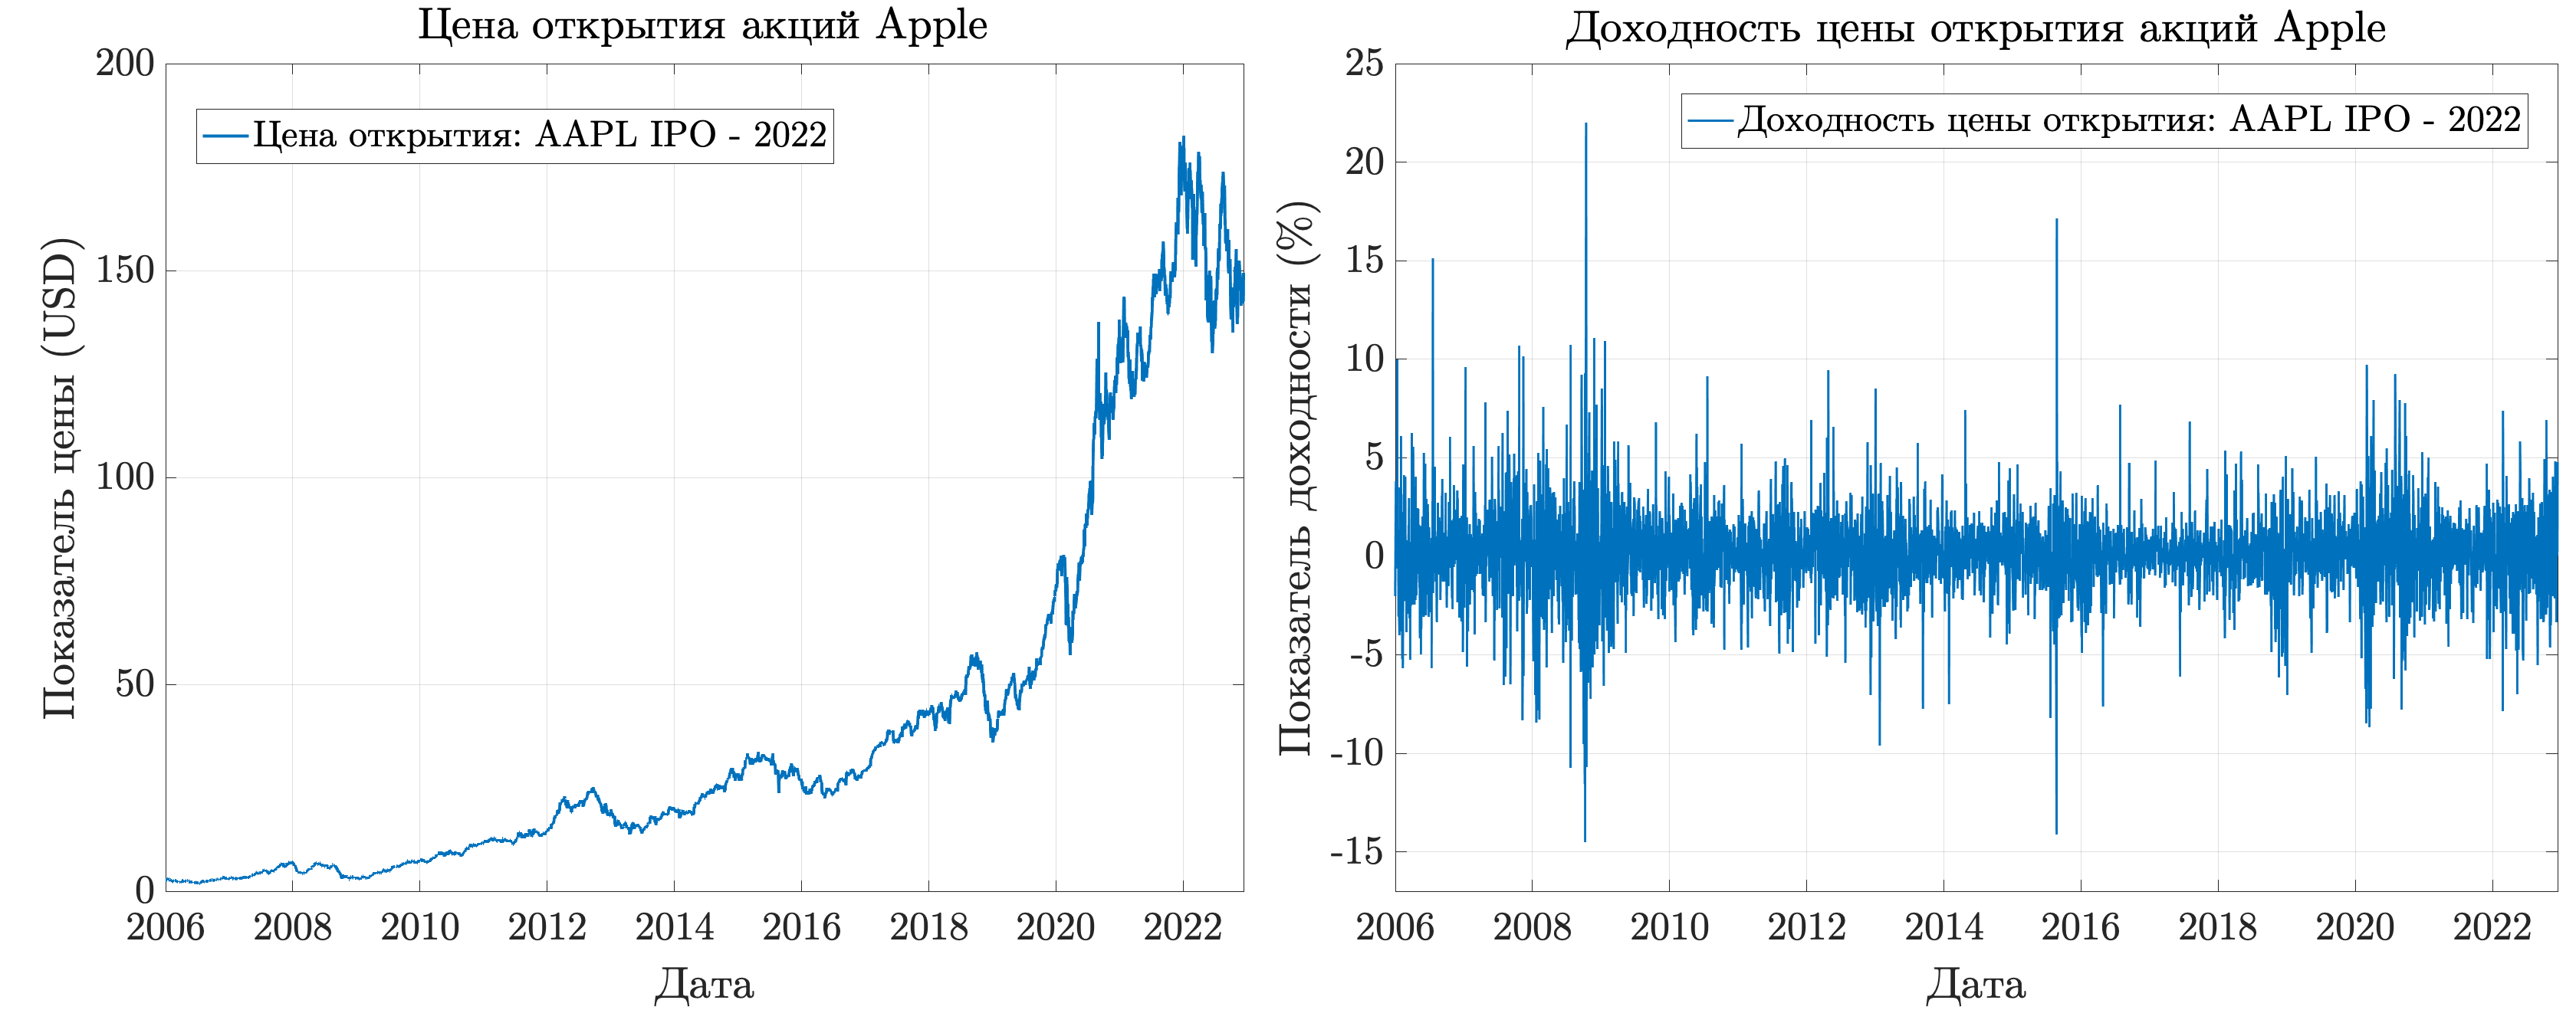
\includegraphics[width=17cm]{returns pictures/apple_prices_returns.png}
	\caption{График цены открытия и доходности Apple (IPO - 2022)}
	\label{fig::apple_prices_returns}
\end{figure}
\noindent А теперь графики амплитуд соответственно. Глядя на график (\ref{fig::amplitudes_apple_prices_returns}), видим, что показатель цены акции не содержит в себе значимой частотной информации, то есть выделить некоторые наиболее сильно <<звучащие>> частоты не удалось. Пик в самом начале (и симметричный ему в конце) отвечает за среднее значение, так как, подставляя в выражение (\myref{equation::fourier_approximation}) $k = 0$, получаем константу. Однако, исходя из амплитуд доходности, понимаем, что они, в свою очередь, включают в себя достаточно большое количество информации о частотах. Но пока что это еще не успех, так как, основываясь на том же графике (\ref{fig::amplitudes_apple_prices_returns}), получается, что значимы все частоты. 
\begin{figure}[H]
	\centering
	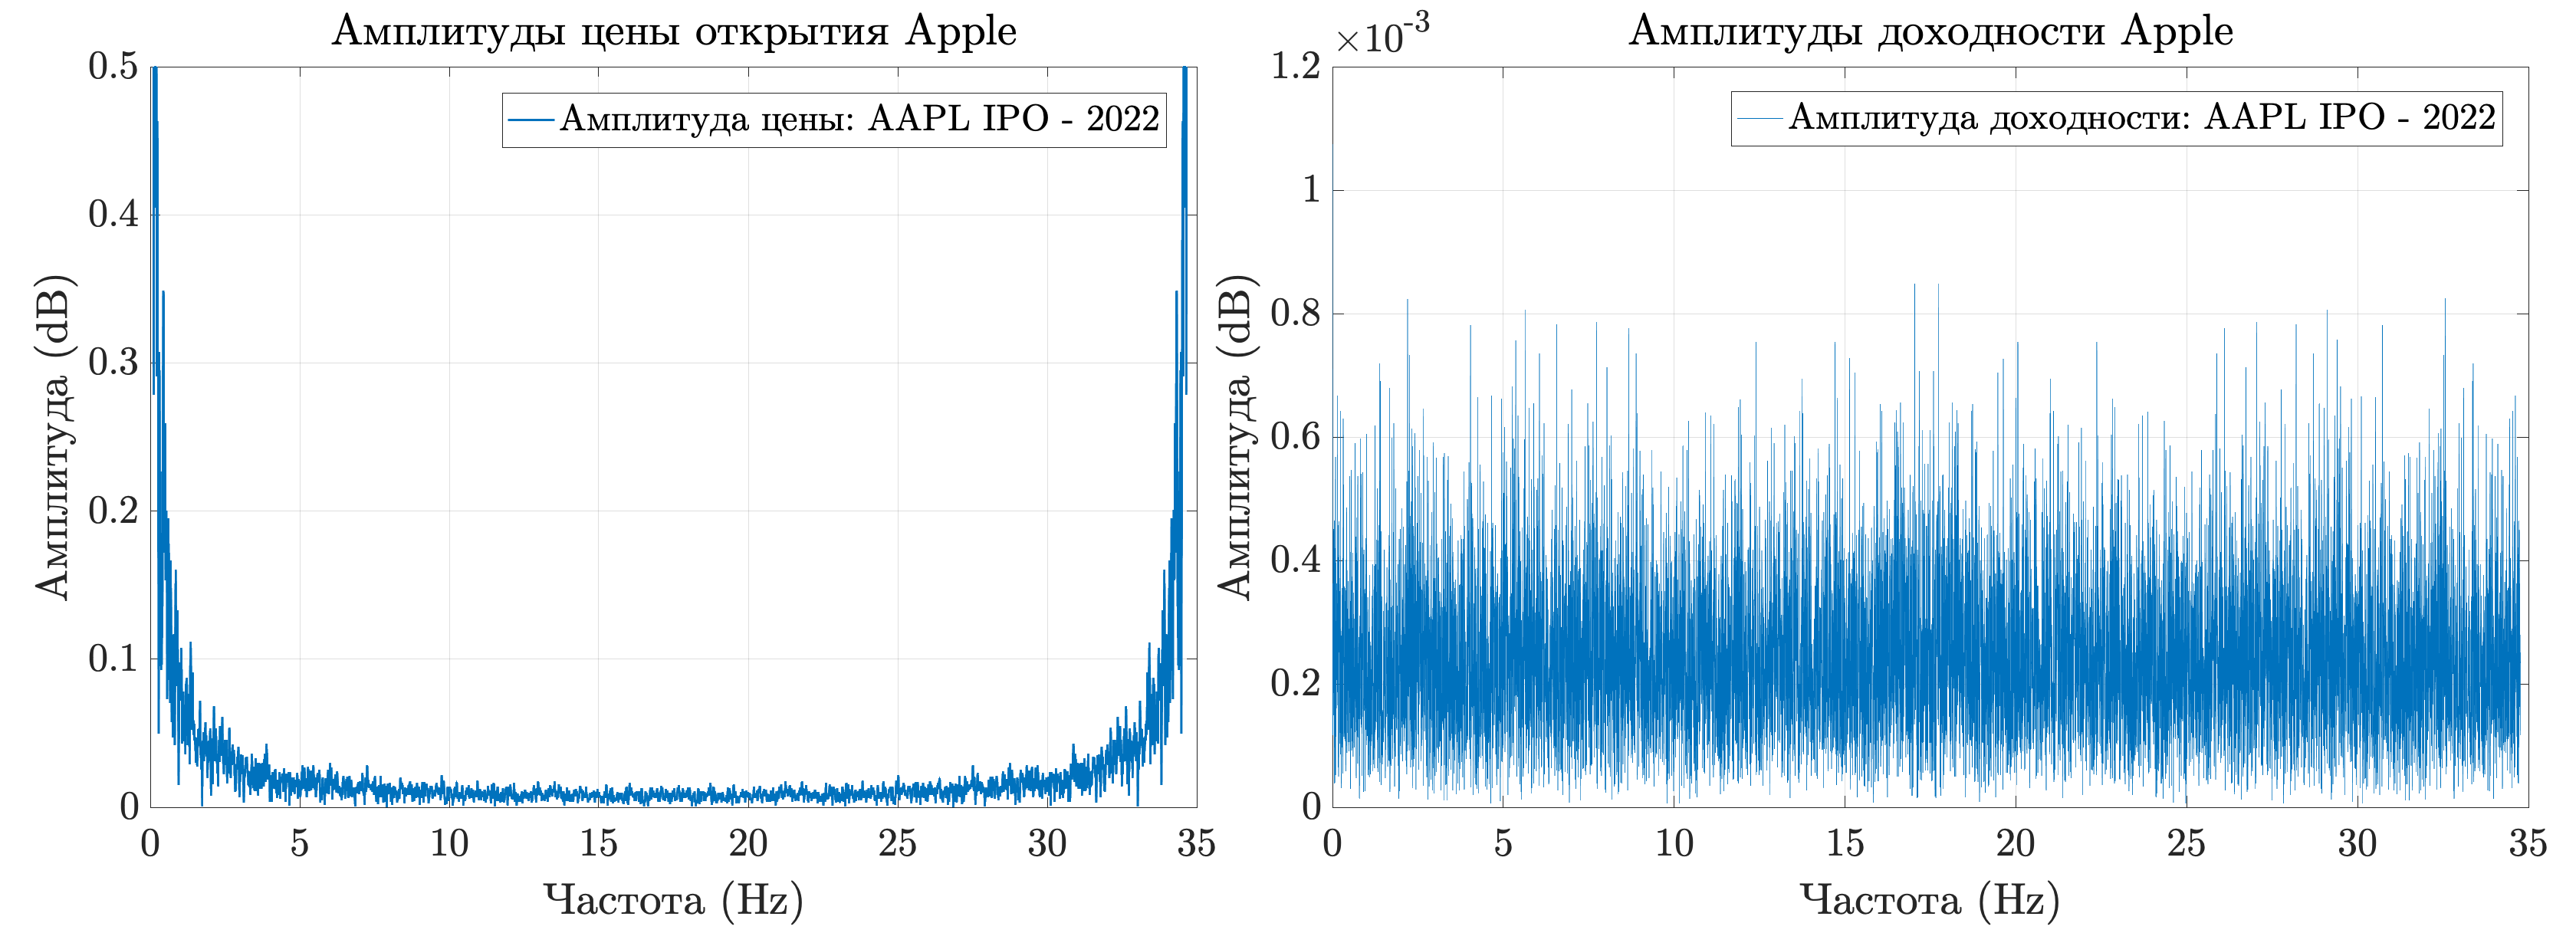
\includegraphics[width=17cm]{time frequency/amplitudes_apple_prices_returns.png}
	\caption{График амплитуд цены открытия и доходности Apple (IPO - 2022)}
	\label{fig::amplitudes_apple_prices_returns}
\end{figure}
Глядя же на график (\ref{fig::apple_prices_returns}) очевидно, что в <<сигнале>> доходности частота разная для каждого периода времени. Это характеризуется разной степенью волатильности показателя доходности, как уже отмечалось в (\myref{link::garch_block}), а также (\myref{link::figarch}). Иными словами, ранее говорилось об <<условной гетероскедастичности>>, а теперь говорится о <<непостоянстве частот во времени>>.

Таким образом, получается, что анализ Фурье применим к анализу финансовых рядов (в особенности доходностей), однако, исходя из самих значений сигнала, нарушается главная предпосылка - постоянство частот во времени. Следовательно, необходим подход, основанный на анализе Фурье, но учитывающий при это непостоянство частот. Это и есть Wavelet анализ (см. \myref{link::wavelet_analysis}), речь о котором идет далее.
\subsubsubsection{Анализ wavelet} \label{link::wavelet_analysis}
\\\\
\subsubsubsection{Пример: Wavelet удаление шума}
\begin{figure}[H]
	\centering
	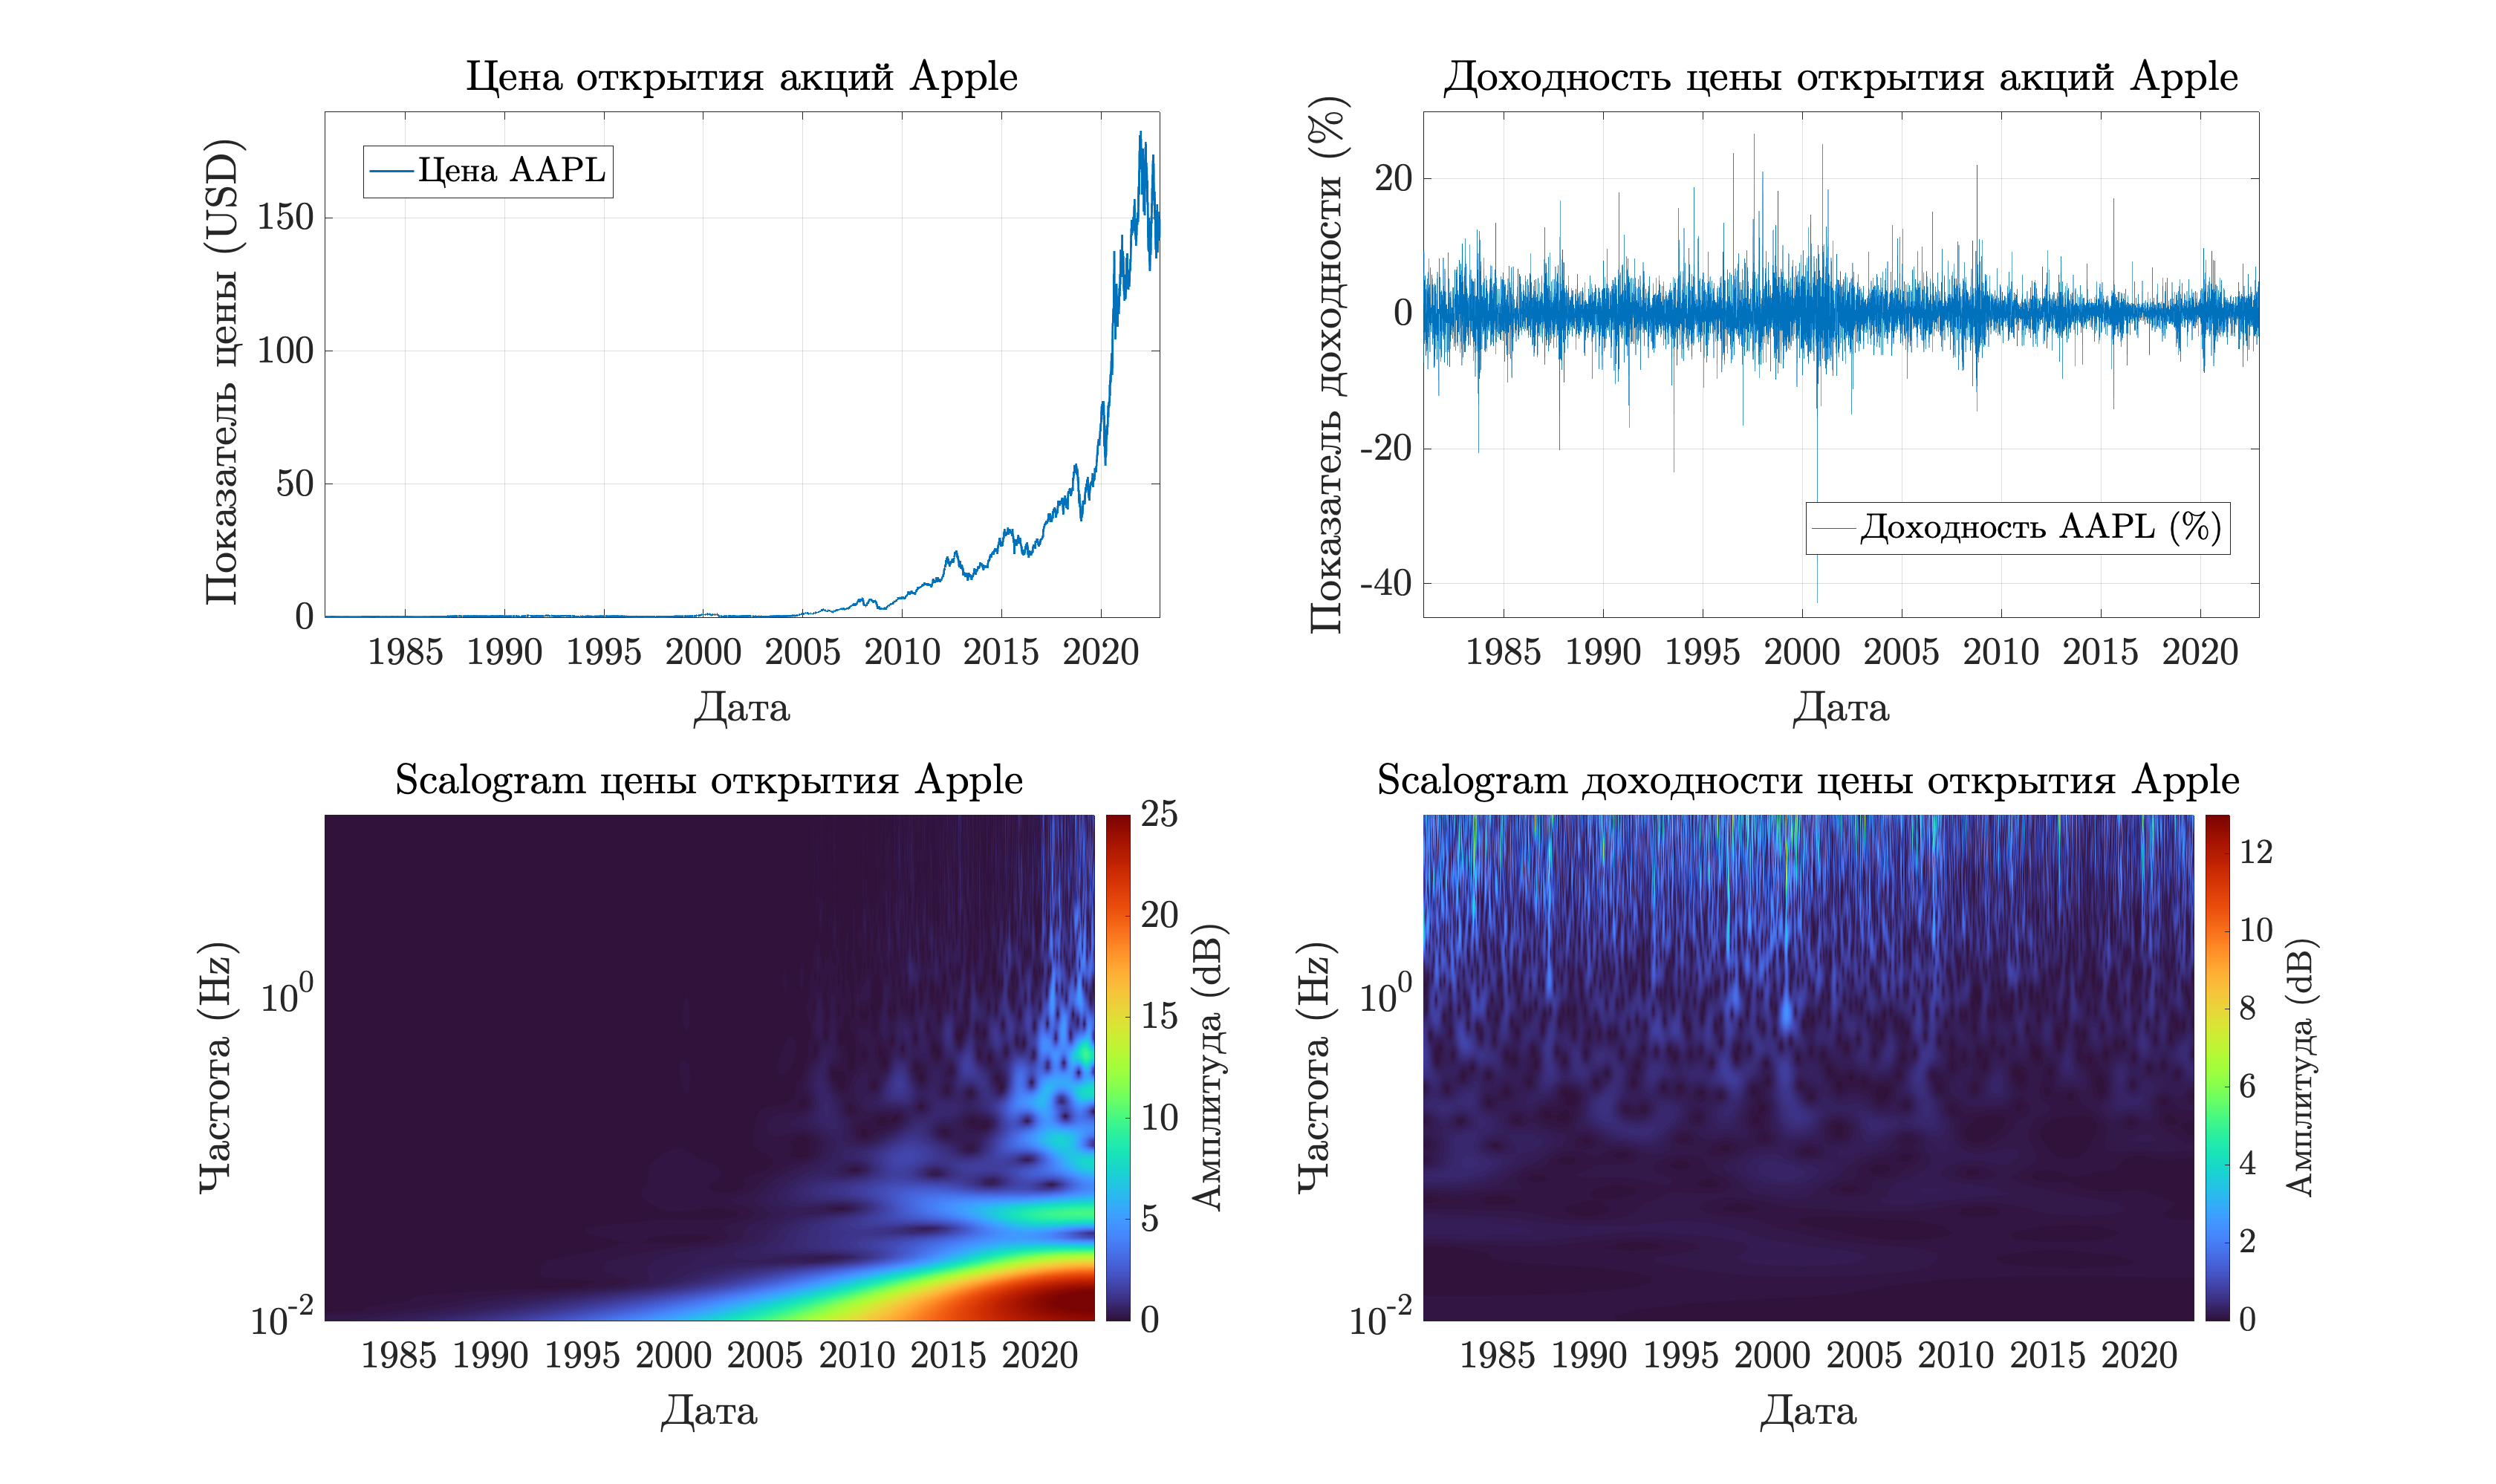
\includegraphics[width= 1.05\textwidth]{time frequency/scalogram_plots.png}
	\caption{График scalogram цены открытия и доходности Apple (IPO - 2022)}
	\label{fig::wavelet_example}
\end{figure}
Интересно, что теперь, по сравнению с анализом Фурье, четко выделено отсутствие какой-либо частотной информации для цен Apple, однако четко прослеживается очень большой ее объем в доходностях. Более того, наблюдая за негативными пиками в доходности, видим, что пики, падающие ниже $-20$ имеют четко выраженную лаговую структуру. В верхней части scalogram для доходностей существуют яркие пики, которые аккурат влекут за собой падение доходности, что аналогично предыдущему подтверждает наличие частотной информации в доходностях акций.

Однако конкретно данный алгоритм, как и преобразование Фурье, не получится использовать для прогнозирования, таким образом, их (алгоритмов) главная задача в настоящей работе - обеспечение очистки данных от шумовых компонент, обусловленных как погрешностью, так и временным лагом между наблюдениями - в случае Apple - это примерно $35$ часов.

Теперь приводим пример работы алгоритма очистки посредством применения WA (Wavelet Analysis). Рассматриваем все ту же функцию (\myref{link::illustr_func}).
\begin{figure}[H]
	\centering
	\begin{tikzpicture}
		\begin{axis}[
			grid = both,
			legend pos = north west,
			minor tick num = 1,
			major grid style = {lightgray},
			minor grid style = {lightgray!25},
			%title= {},
			width = \textwidth,
			height = 0.45 \textwidth,
			xmin=-5, xmax=5,
			ymin=-4, ymax=7.5,
			line width=0.3mm
			]
			
			\addplot[color = orange, line width = 0.035cm] table [
			x=x, 
			y=y_clean, 
			col sep=comma,
			mark={},
			] {./source/source_csv/Illustration data/wavelet/wavelet_example_denoising.csv};
			
			\addplot[opacity = 0.25, color = blue] table [
			x=x, 
			y=y_initial, 
			col sep=comma,
			mark={},
			] {./source/source_csv/Illustration data/wavelet/wavelet_example_denoising.csv};
			
			\addplot[domain = -5:5,
			samples = 300,
			color = teal,
			smooth,
			line width = 0.025cm,] {sin(deg(5 * x)) + 1 / 4 * (x^2)};
			
			\legend{$f(x)$ очищенный, $f(x)$ c шумом, $f(x)$ без шума};
		\end{axis}
	\end{tikzpicture}
	\caption{Очистка ряда от шума посредством преобразования Wavelet}
\end{figure}
Ошибка $\text{RMSE} = 0.7649$, что заметно больше, чем в случае применения метода MSSA, где ошибка $\text{RMSE} = 0.1744$ (\myref{link::mssa}). Таким образом, получаем, что для очистки от шума лучше использовать MSSA. Но в таком случае, появляется вопрос \textbf{Q}: Зачем весь этот метод тут, если, применяя его, не получается как прогнозировать (без специальных дополнительных предпосылок или теоретических выкладок, как, например, в статье \cite{schluter2010using}), так и лучше, чем MSSA очищать от шума (не строгое утверждение, а лишь основа на результате исследования настоящей работы)? \textbf{A}: Ответ присутствует в блоке (\myref{link::wavelet_nets}), где приводится описание применения Wavelet анализа к построению <<сетевых>> архитектур. Под <<сетевыми>> подразумеваются нейронные сети.

Таким образом, пока что вышеупомянутые методы Фурье и Wavelet преобразования остаются лишь прикладными к другим методам (это верно только для настоящей работы), так как напрямую для прогнозирования не применяются, однако это ничего не говорит об их качестве работы с анализируемыми данными. Далее переходим к описанию наиболее важной части текущего исследования, посвященной нейросетевому подходу к решению задачи прогнозирования показателей.